\documentclass[1p]{elsarticle_modified}
%\bibliographystyle{elsarticle-num}

%\usepackage[colorlinks]{hyperref}
%\usepackage{abbrmath_seonhwa} %\Abb, \Ascr, \Acal ,\Abf, \Afrak
\usepackage{amsfonts}
\usepackage{amssymb}
\usepackage{amsmath}
\usepackage{amsthm}
\usepackage{scalefnt}
\usepackage{amsbsy}
\usepackage{kotex}
\usepackage{caption}
\usepackage{subfig}
\usepackage{color}
\usepackage{graphicx}
\usepackage{xcolor} %% white, black, red, green, blue, cyan, magenta, yellow
\usepackage{float}
\usepackage{setspace}
\usepackage{hyperref}

\usepackage{tikz}
\usetikzlibrary{arrows}

\usepackage{multirow}
\usepackage{array} % fixed length table
\usepackage{hhline}

%%%%%%%%%%%%%%%%%%%%%
\makeatletter
\renewcommand*\env@matrix[1][\arraystretch]{%
	\edef\arraystretch{#1}%
	\hskip -\arraycolsep
	\let\@ifnextchar\new@ifnextchar
	\array{*\c@MaxMatrixCols c}}
\makeatother %https://tex.stackexchange.com/questions/14071/how-can-i-increase-the-line-spacing-in-a-matrix
%%%%%%%%%%%%%%%

\usepackage[normalem]{ulem}

\newcommand{\msout}[1]{\ifmmode\text{\sout{\ensuremath{#1}}}\else\sout{#1}\fi}
%SOURCE: \msout is \stkout macro in https://tex.stackexchange.com/questions/20609/strikeout-in-math-mode

\newcommand{\cancel}[1]{
	\ifmmode
	{\color{red}\msout{#1}}
	\else
	{\color{red}\sout{#1}}
	\fi
}

\newcommand{\add}[1]{
	{\color{blue}\uwave{#1}}
}

\newcommand{\replace}[2]{
	\ifmmode
	{\color{red}\msout{#1}}{\color{blue}\uwave{#2}}
	\else
	{\color{red}\sout{#1}}{\color{blue}\uwave{#2}}
	\fi
}

\newcommand{\Sol}{\mathcal{S}} %segment
\newcommand{\D}{D} %diagram
\newcommand{\A}{\mathcal{A}} %arc


%%%%%%%%%%%%%%%%%%%%%%%%%%%%%5 test

\def\sl{\operatorname{\textup{SL}}(2,\Cbb)}
\def\psl{\operatorname{\textup{PSL}}(2,\Cbb)}
\def\quan{\mkern 1mu \triangleright \mkern 1mu}

\theoremstyle{definition}
\newtheorem{thm}{Theorem}[section]
\newtheorem{prop}[thm]{Proposition}
\newtheorem{lem}[thm]{Lemma}
\newtheorem{ques}[thm]{Question}
\newtheorem{cor}[thm]{Corollary}
\newtheorem{defn}[thm]{Definition}
\newtheorem{exam}[thm]{Example}
\newtheorem{rmk}[thm]{Remark}
\newtheorem{alg}[thm]{Algorithm}

\newcommand{\I}{\sqrt{-1}}
\begin{document}

%\begin{frontmatter}
%
%\title{Boundary parabolic representations of knots up to 8 crossings}
%
%%% Group authors per affiliation:
%\author{Yunhi Cho} 
%\address{Department of Mathematics, University of Seoul, Seoul, Korea}
%\ead{yhcho@uos.ac.kr}
%
%
%\author{Seonhwa Kim} %\fnref{s_kim}}
%\address{Center for Geometry and Physics, Institute for Basic Science, Pohang, 37673, Korea}
%\ead{ryeona17@ibs.re.kr}
%
%\author{Hyuk Kim}
%\address{Department of Mathematical Sciences, Seoul National University, Seoul 08826, Korea}
%\ead{hyukkim@snu.ac.kr}
%
%\author{Seokbeom Yoon}
%\address{Department of Mathematical Sciences, Seoul National University, Seoul, 08826,  Korea}
%\ead{sbyoon15@snu.ac.kr}
%
%\begin{abstract}
%We find all boundary parabolic representation of knots up to 8 crossings.
%
%\end{abstract}
%\begin{keyword}
%    \MSC[2010] 57M25 
%\end{keyword}
%
%\end{frontmatter}

%\linenumbers
%\tableofcontents
%
\newcommand\colored[1]{\textcolor{white}{\rule[-0.35ex]{0.8em}{1.4ex}}\kern-0.8em\color{red} #1}%
%\newcommand\colored[1]{\textcolor{white}{ #1}\kern-2.17ex	\textcolor{white}{ #1}\kern-1.81ex	\textcolor{white}{ #1}\kern-2.15ex\color{red}#1	}

{\Large $\underline{11a_{236}~(K11a_{236})}$}

\setlength{\tabcolsep}{10pt}
\renewcommand{\arraystretch}{1.6}
\vspace{1cm}\begin{tabular}{m{100pt}>{\centering\arraybackslash}m{274pt}}
\multirow{5}{120pt}{
	\centering
	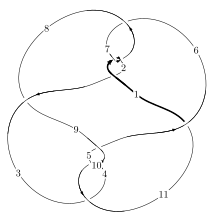
\includegraphics[width=112pt]{../../../GIT/diagram.site/Diagrams/png/485_11a_236.png}\\
\ \ \ A knot diagram\footnotemark}&
\allowdisplaybreaks
\textbf{Linearized knot diagam} \\
\cline{2-2}
 &
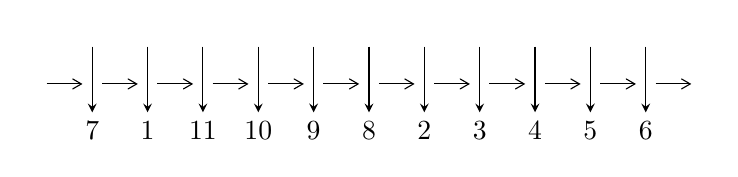
\begin{tikzpicture}[x=20pt, y=17pt]
	% nodes
	\node (C0) at (0, 0) {};
	\node (C1) at (1, 0) {};
	\node (C1U) at (1, +1) {};
	\node (C1D) at (1, -1) {7};

	\node (C2) at (2, 0) {};
	\node (C2U) at (2, +1) {};
	\node (C2D) at (2, -1) {1};

	\node (C3) at (3, 0) {};
	\node (C3U) at (3, +1) {};
	\node (C3D) at (3, -1) {11};

	\node (C4) at (4, 0) {};
	\node (C4U) at (4, +1) {};
	\node (C4D) at (4, -1) {10};

	\node (C5) at (5, 0) {};
	\node (C5U) at (5, +1) {};
	\node (C5D) at (5, -1) {9};

	\node (C6) at (6, 0) {};
	\node (C6U) at (6, +1) {};
	\node (C6D) at (6, -1) {8};

	\node (C7) at (7, 0) {};
	\node (C7U) at (7, +1) {};
	\node (C7D) at (7, -1) {2};

	\node (C8) at (8, 0) {};
	\node (C8U) at (8, +1) {};
	\node (C8D) at (8, -1) {3};

	\node (C9) at (9, 0) {};
	\node (C9U) at (9, +1) {};
	\node (C9D) at (9, -1) {4};

	\node (C10) at (10, 0) {};
	\node (C10U) at (10, +1) {};
	\node (C10D) at (10, -1) {5};

	\node (C11) at (11, 0) {};
	\node (C11U) at (11, +1) {};
	\node (C11D) at (11, -1) {6};
	\node (C12) at (12, 0) {};

	% arrows
	\draw[->,>={angle 60}]
	(C0) edge (C1) (C1) edge (C2) (C2) edge (C3) (C3) edge (C4) (C4) edge (C5) (C5) edge (C6) (C6) edge (C7) (C7) edge (C8) (C8) edge (C9) (C9) edge (C10) (C10) edge (C11) (C11) edge (C12) ;	\draw[->,>=stealth]
	(C1U) edge (C1D) (C2U) edge (C2D) (C3U) edge (C3D) (C4U) edge (C4D) (C5U) edge (C5D) (C6U) edge (C6D) (C7U) edge (C7D) (C8U) edge (C8D) (C9U) edge (C9D) (C10U) edge (C10D) (C11U) edge (C11D) ;
	\end{tikzpicture} \\
\hhline{~~} \\& 
\textbf{Solving Sequence} \\ \cline{2-2} 
 &
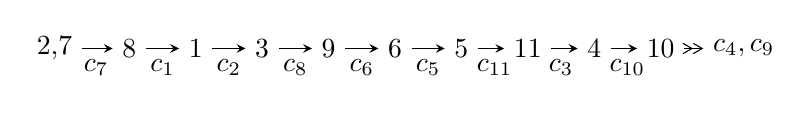
\begin{tikzpicture}[x=24pt, y=7pt]
	% node
	\node (A0) at (-1/8, 0) {2,7};
	\node (A1) at (1, 0) {8};
	\node (A2) at (2, 0) {1};
	\node (A3) at (3, 0) {3};
	\node (A4) at (4, 0) {9};
	\node (A5) at (5, 0) {6};
	\node (A6) at (6, 0) {5};
	\node (A7) at (7, 0) {11};
	\node (A8) at (8, 0) {4};
	\node (A9) at (9, 0) {10};
	\node (C1) at (1/2, -1) {$c_{7}$};
	\node (C2) at (3/2, -1) {$c_{1}$};
	\node (C3) at (5/2, -1) {$c_{2}$};
	\node (C4) at (7/2, -1) {$c_{8}$};
	\node (C5) at (9/2, -1) {$c_{6}$};
	\node (C6) at (11/2, -1) {$c_{5}$};
	\node (C7) at (13/2, -1) {$c_{11}$};
	\node (C8) at (15/2, -1) {$c_{3}$};
	\node (C9) at (17/2, -1) {$c_{10}$};
	\node (A10) at (41/4, 0) {$c_{4},c_{9}$};

	% edge
	\draw[->,>=stealth]	
	(A0) edge (A1) (A1) edge (A2) (A2) edge (A3) (A3) edge (A4) (A4) edge (A5) (A5) edge (A6) (A6) edge (A7) (A7) edge (A8) (A8) edge (A9) ;
	\draw[->>,>={angle 60}]	
	(A9) edge (A10);
\end{tikzpicture} \\ 

\end{tabular} \\

\footnotetext{
The image of knot diagram is generated by the software ``\textbf{Draw programme}" developed by Andrew Bartholomew(\url{http://www.layer8.co.uk/maths/draw/index.htm\#Running-draw}), where we modified some parts for our purpose(\url{https://github.com/CATsTAILs/LinksPainter}).
}\phantom \\ \newline 
\centering \textbf{Ideals for irreducible components\footnotemark of $X_{\text{par}}$} 
 
\begin{align*}
I^u_{1}&=\langle 
u^{48}-2 u^{47}+\cdots-4 u+1\rangle \\
I^u_{2}&=\langle 
u+1\rangle \\
\\
\end{align*}
\raggedright * 2 irreducible components of $\dim_{\mathbb{C}}=0$, with total 49 representations.\\
\footnotetext{All coefficients of polynomials are rational numbers. But the coefficients are sometimes approximated in decimal forms when there is not enough margin.}
\newpage
\renewcommand{\arraystretch}{1}
\centering \section*{I. $I^u_{1}= \langle u^{48}-2 u^{47}+\cdots-4 u+1 \rangle$}
\flushleft \textbf{(i) Arc colorings}\\
\begin{tabular}{m{7pt} m{180pt} m{7pt} m{180pt} }
\flushright $a_{2}=$&$\begin{pmatrix}0\\u\end{pmatrix}$ \\
\flushright $a_{7}=$&$\begin{pmatrix}1\\0\end{pmatrix}$ \\
\flushright $a_{8}=$&$\begin{pmatrix}1\\u^2\end{pmatrix}$ \\
\flushright $a_{1}=$&$\begin{pmatrix}u\\u\end{pmatrix}$ \\
\flushright $a_{3}=$&$\begin{pmatrix}- u^3\\- u^3+u\end{pmatrix}$ \\
\flushright $a_{9}=$&$\begin{pmatrix}- u^8+u^6- u^4+1\\- u^8+2 u^6-2 u^4+2 u^2\end{pmatrix}$ \\
\flushright $a_{6}=$&$\begin{pmatrix}- u^2+1\\- u^4\end{pmatrix}$ \\
\flushright $a_{5}=$&$\begin{pmatrix}- u^{20}+3 u^{18}-7 u^{16}+10 u^{14}-10 u^{12}+7 u^{10}- u^8-2 u^6+3 u^4-3 u^2+1\\- u^{20}+4 u^{18}-10 u^{16}+18 u^{14}-23 u^{12}+24 u^{10}-18 u^8+10 u^6-5 u^4\end{pmatrix}$ \\
\flushright $a_{11}=$&$\begin{pmatrix}- u^7+2 u^5-2 u^3+2 u\\- u^9+u^7- u^5+u\end{pmatrix}$ \\
\flushright $a_{4}=$&$\begin{pmatrix}- u^{19}+4 u^{17}-10 u^{15}+18 u^{13}-23 u^{11}+24 u^9-18 u^7+10 u^5-5 u^3\\- u^{21}+3 u^{19}-7 u^{17}+10 u^{15}-10 u^{13}+7 u^{11}- u^9-2 u^7+3 u^5-3 u^3+u\end{pmatrix}$ \\
\flushright $a_{10}=$&$\begin{pmatrix}-2 u^{47}+3 u^{46}+\cdots-4 u+2\\- u^{47}+3 u^{46}+\cdots-6 u+2\end{pmatrix}$\\ \flushright $a_{10}=$&$\begin{pmatrix}-2 u^{47}+3 u^{46}+\cdots-4 u+2\\- u^{47}+3 u^{46}+\cdots-6 u+2\end{pmatrix}$\\&\end{tabular}
\flushleft \textbf{(ii) Obstruction class $= -1$}\\~\\
\flushleft \textbf{(iii) Cusp Shapes $= 8 u^{47}-12 u^{46}+\cdots+28 u-26$}\\~\\
\newpage\renewcommand{\arraystretch}{1}
\flushleft \textbf{(iv) u-Polynomials at the component}\newline \\
\begin{tabular}{m{50pt}|m{274pt}}
Crossings & \hspace{64pt}u-Polynomials at each crossing \\
\hline $$\begin{aligned}c_{1},c_{7}\end{aligned}$$&$\begin{aligned}
&u^{48}+2 u^{47}+\cdots+4 u+1
\end{aligned}$\\
\hline $$\begin{aligned}c_{2},c_{6}\end{aligned}$$&$\begin{aligned}
&u^{48}+16 u^{47}+\cdots+8 u+1
\end{aligned}$\\
\hline $$\begin{aligned}c_{3},c_{5}\end{aligned}$$&$\begin{aligned}
&u^{48}-3 u^{47}+\cdots-20 u^2+1
\end{aligned}$\\
\hline $$\begin{aligned}c_{4},c_{9},c_{10}\end{aligned}$$&$\begin{aligned}
&u^{48}+2 u^{47}+\cdots+4 u+1
\end{aligned}$\\
\hline $$\begin{aligned}c_{8},c_{11}\end{aligned}$$&$\begin{aligned}
&u^{48}-14 u^{46}+\cdots+4 u+1
\end{aligned}$\\
\hline
\end{tabular}\\~\\
\newpage\renewcommand{\arraystretch}{1}
\flushleft \textbf{(v) Riley Polynomials at the component}\newline \\
\begin{tabular}{m{50pt}|m{274pt}}
Crossings & \hspace{64pt}Riley Polynomials at each crossing \\
\hline $$\begin{aligned}c_{1},c_{7}\end{aligned}$$&$\begin{aligned}
&y^{48}-16 y^{47}+\cdots-8 y+1
\end{aligned}$\\
\hline $$\begin{aligned}c_{2},c_{6}\end{aligned}$$&$\begin{aligned}
&y^{48}+32 y^{47}+\cdots-8 y+1
\end{aligned}$\\
\hline $$\begin{aligned}c_{3},c_{5}\end{aligned}$$&$\begin{aligned}
&y^{48}+27 y^{47}+\cdots-40 y+1
\end{aligned}$\\
\hline $$\begin{aligned}c_{4},c_{9},c_{10}\end{aligned}$$&$\begin{aligned}
&y^{48}-40 y^{47}+\cdots-8 y+1
\end{aligned}$\\
\hline $$\begin{aligned}c_{8},c_{11}\end{aligned}$$&$\begin{aligned}
&y^{48}-28 y^{47}+\cdots+72 y+1
\end{aligned}$\\
\hline
\end{tabular}\\~\\
\newpage\flushleft \textbf{(vi) Complex Volumes and Cusp Shapes}
$$\begin{array}{c|c|c}  
\text{Solutions to }I^u_{1}& \I (\text{vol} + \sqrt{-1}CS) & \text{Cusp shape}\\
 \hline 
\begin{aligned}
u &= \phantom{-}0.882555 + 0.461026 I\end{aligned}
 & -3.01031 - 4.88758 I & -15.6251 + 6.5404 I \\ \hline\begin{aligned}
u &= \phantom{-}0.882555 - 0.461026 I\end{aligned}
 & -3.01031 + 4.88758 I & -15.6251 - 6.5404 I \\ \hline\begin{aligned}
u &= \phantom{-}0.665767 + 0.762214 I\end{aligned}
 & \phantom{-}0.632478 + 0.108144 I & -9.55124 + 0.86883 I \\ \hline\begin{aligned}
u &= \phantom{-}0.665767 - 0.762214 I\end{aligned}
 & \phantom{-}0.632478 - 0.108144 I & -9.55124 - 0.86883 I \\ \hline\begin{aligned}
u &= -0.639372 + 0.784790 I\end{aligned}
 & \phantom{-}3.51281 - 4.08944 I & -6.57921 + 3.06594 I \\ \hline\begin{aligned}
u &= -0.639372 - 0.784790 I\end{aligned}
 & \phantom{-}3.51281 + 4.08944 I & -6.57921 - 3.06594 I \\ \hline\begin{aligned}
u &= \phantom{-}0.624433 + 0.797000 I\end{aligned}
 & -1.18842 + 8.10290 I & -11.33189 - 4.69039 I \\ \hline\begin{aligned}
u &= \phantom{-}0.624433 - 0.797000 I\end{aligned}
 & -1.18842 - 8.10290 I & -11.33189 + 4.69039 I \\ \hline\begin{aligned}
u &= -0.785703 + 0.584322 I\end{aligned}
 & \phantom{-}1.37338 + 2.15146 I & -8.25248 - 5.45590 I \\ \hline\begin{aligned}
u &= -0.785703 - 0.584322 I\end{aligned}
 & \phantom{-}1.37338 - 2.15146 I & -8.25248 + 5.45590 I \\ \hline\begin{aligned}
u &= -1.02158\phantom{ +0.000000I}\end{aligned}
 & -4.93269\phantom{ +0.000000I} & -18.1530\phantom{ +0.000000I} \\ \hline\begin{aligned}
u &= \phantom{-}0.644420 + 0.678291 I\end{aligned}
 & \phantom{-}0.048446 + 0.560613 I & -11.68780 - 1.95261 I \\ \hline\begin{aligned}
u &= \phantom{-}0.644420 - 0.678291 I\end{aligned}
 & \phantom{-}0.048446 - 0.560613 I & -11.68780 + 1.95261 I \\ \hline\begin{aligned}
u &= \phantom{-}1.070420 + 0.070047 I\end{aligned}
 & -2.46715 - 3.58742 I & -13.8838 + 4.2943 I \\ \hline\begin{aligned}
u &= \phantom{-}1.070420 - 0.070047 I\end{aligned}
 & -2.46715 + 3.58742 I & -13.8838 - 4.2943 I \\ \hline\begin{aligned}
u &= -0.921125\phantom{ +0.000000I}\end{aligned}
 & -4.91974\phantom{ +0.000000I} & -18.6280\phantom{ +0.000000I} \\ \hline\begin{aligned}
u &= -0.555627 + 0.727194 I\end{aligned}
 & -5.98604 - 1.18604 I & -15.5397 + 0.4606 I \\ \hline\begin{aligned}
u &= -0.555627 - 0.727194 I\end{aligned}
 & -5.98604 + 1.18604 I & -15.5397 - 0.4606 I \\ \hline\begin{aligned}
u &= -1.093390 + 0.071584 I\end{aligned}
 & -7.29017 + 7.41299 I & -18.4799 - 5.5389 I \\ \hline\begin{aligned}
u &= -1.093390 - 0.071584 I\end{aligned}
 & -7.29017 - 7.41299 I & -18.4799 + 5.5389 I \\ \hline\begin{aligned}
u &= \phantom{-}1.09915\phantom{ +0.000000I}\end{aligned}
 & -11.4368\phantom{ +0.000000I} & -21.8600\phantom{ +0.000000I} \\ \hline\begin{aligned}
u &= -0.841196 + 0.750320 I\end{aligned}
 & \phantom{-}3.16432 - 1.24428 I & -8.04097 + 0.56162 I \\ \hline\begin{aligned}
u &= -0.841196 - 0.750320 I\end{aligned}
 & \phantom{-}3.16432 + 1.24428 I & -8.04097 - 0.56162 I \\ \hline\begin{aligned}
u &= \phantom{-}0.863763 + 0.744913 I\end{aligned}
 & \phantom{-}6.99140 - 2.82021 I & -3.95134 + 3.08292 I \\ \hline\begin{aligned}
u &= \phantom{-}0.863763 - 0.744913 I\end{aligned}
 & \phantom{-}6.99140 + 2.82021 I & -3.95134 - 3.08292 I \\ \hline\begin{aligned}
u &= -0.977993 + 0.605871 I\end{aligned}
 & \phantom{-}0.66805 + 2.46888 I & -10.26548 - 1.31520 I \\ \hline\begin{aligned}
u &= -0.977993 - 0.605871 I\end{aligned}
 & \phantom{-}0.66805 - 2.46888 I & -10.26548 + 1.31520 I \\ \hline\begin{aligned}
u &= -0.885079 + 0.741658 I\end{aligned}
 & \phantom{-}3.03130 + 6.89085 I & -8.49212 - 6.46442 I \\ \hline\begin{aligned}
u &= -0.885079 - 0.741658 I\end{aligned}
 & \phantom{-}3.03130 - 6.89085 I & -8.49212 + 6.46442 I \\ \hline\begin{aligned}
u &= \phantom{-}1.009840 + 0.589266 I\end{aligned}
 & -4.16473 + 0.96747 I & -15.6034 + 0. I\phantom{ +0.000000I}\\
 \hline 
 \end{array}$$\newpage$$\begin{array}{c|c|c}  
\text{Solutions to }I^u_{1}& \I (\text{vol} + \sqrt{-1}CS) & \text{Cusp shape}\\
 \hline 
\begin{aligned}
u &= \phantom{-}1.009840 - 0.589266 I\end{aligned}
 & -4.16473 - 0.96747 I & -15.6034 + 0. I\phantom{ +0.000000I} \\ \hline\begin{aligned}
u &= \phantom{-}0.996479 + 0.655041 I\end{aligned}
 & -0.98972 - 5.75638 I & -13.3076 + 6.8650 I \\ \hline\begin{aligned}
u &= \phantom{-}0.996479 - 0.655041 I\end{aligned}
 & -0.98972 + 5.75638 I & -13.3076 - 6.8650 I \\ \hline\begin{aligned}
u &= -1.031620 + 0.650416 I\end{aligned}
 & -7.35665 + 6.46067 I & -17.5687 - 5.3712 I \\ \hline\begin{aligned}
u &= -1.031620 - 0.650416 I\end{aligned}
 & -7.35665 - 6.46067 I & -17.5687 + 5.3712 I \\ \hline\begin{aligned}
u &= \phantom{-}1.006860 + 0.688557 I\end{aligned}
 & -0.39402 - 5.62399 I & -11.59767 + 4.05733 I \\ \hline\begin{aligned}
u &= \phantom{-}1.006860 - 0.688557 I\end{aligned}
 & -0.39402 + 5.62399 I & -11.59767 - 4.05733 I \\ \hline\begin{aligned}
u &= -1.024260 + 0.692231 I\end{aligned}
 & \phantom{-}2.35847 + 9.67537 I & -8.68198 - 7.82216 I \\ \hline\begin{aligned}
u &= -1.024260 - 0.692231 I\end{aligned}
 & \phantom{-}2.35847 - 9.67537 I & -8.68198 + 7.82216 I \\ \hline\begin{aligned}
u &= \phantom{-}1.033900 + 0.692265 I\end{aligned}
 & -2.41639 - 13.71870 I & -13.3452 + 9.2783 I \\ \hline\begin{aligned}
u &= \phantom{-}1.033900 - 0.692265 I\end{aligned}
 & -2.41639 + 13.71870 I & -13.3452 - 9.2783 I \\ \hline\begin{aligned}
u &= \phantom{-}0.376949 + 0.637932 I\end{aligned}
 & -2.56451 - 5.60912 I & -12.01724 + 5.48028 I \\ \hline\begin{aligned}
u &= \phantom{-}0.376949 - 0.637932 I\end{aligned}
 & -2.56451 + 5.60912 I & -12.01724 - 5.48028 I \\ \hline\begin{aligned}
u &= -0.339798 + 0.564531 I\end{aligned}
 & \phantom{-}1.97900 + 1.93404 I & -6.47322 - 4.04899 I \\ \hline\begin{aligned}
u &= -0.339798 - 0.564531 I\end{aligned}
 & \phantom{-}1.97900 - 1.93404 I & -6.47322 + 4.04899 I \\ \hline\begin{aligned}
u &= \phantom{-}0.209593 + 0.518446 I\end{aligned}
 & -1.32155 + 1.52053 I & -9.58208 - 0.33085 I \\ \hline\begin{aligned}
u &= \phantom{-}0.209593 - 0.518446 I\end{aligned}
 & -1.32155 - 1.52053 I & -9.58208 + 0.33085 I \\ \hline\begin{aligned}
u &= \phantom{-}0.421695\phantom{ +0.000000I}\end{aligned}
 & -0.568709\phantom{ +0.000000I} & -17.6430\phantom{ +0.000000I}\\
 \hline 
 \end{array}$$\newpage\newpage\renewcommand{\arraystretch}{1}
\centering \section*{II. $I^u_{2}= \langle u+1 \rangle$}
\flushleft \textbf{(i) Arc colorings}\\
\begin{tabular}{m{7pt} m{180pt} m{7pt} m{180pt} }
\flushright $a_{2}=$&$\begin{pmatrix}0\\-1\end{pmatrix}$ \\
\flushright $a_{7}=$&$\begin{pmatrix}1\\0\end{pmatrix}$ \\
\flushright $a_{8}=$&$\begin{pmatrix}1\\1\end{pmatrix}$ \\
\flushright $a_{1}=$&$\begin{pmatrix}-1\\-1\end{pmatrix}$ \\
\flushright $a_{3}=$&$\begin{pmatrix}1\\0\end{pmatrix}$ \\
\flushright $a_{9}=$&$\begin{pmatrix}0\\1\end{pmatrix}$ \\
\flushright $a_{6}=$&$\begin{pmatrix}0\\-1\end{pmatrix}$ \\
\flushright $a_{5}=$&$\begin{pmatrix}0\\-1\end{pmatrix}$ \\
\flushright $a_{11}=$&$\begin{pmatrix}-1\\0\end{pmatrix}$ \\
\flushright $a_{4}=$&$\begin{pmatrix}1\\0\end{pmatrix}$ \\
\flushright $a_{10}=$&$\begin{pmatrix}-1\\1\end{pmatrix}$\\ \flushright $a_{10}=$&$\begin{pmatrix}-1\\1\end{pmatrix}$\\&\end{tabular}
\flushleft \textbf{(ii) Obstruction class $= -1$}\\~\\
\flushleft \textbf{(iii) Cusp Shapes $= -18$}\\~\\
\newpage\renewcommand{\arraystretch}{1}
\flushleft \textbf{(iv) u-Polynomials at the component}\newline \\
\begin{tabular}{m{50pt}|m{274pt}}
Crossings & \hspace{64pt}u-Polynomials at each crossing \\
\hline $$\begin{aligned}c_{1},c_{4},c_{7}\\c_{8},c_{9},c_{10}\\c_{11}\end{aligned}$$&$\begin{aligned}
&u-1
\end{aligned}$\\
\hline $$\begin{aligned}c_{2},c_{6}\end{aligned}$$&$\begin{aligned}
&u+1
\end{aligned}$\\
\hline $$\begin{aligned}c_{3},c_{5}\end{aligned}$$&$\begin{aligned}
&u
\end{aligned}$\\
\hline
\end{tabular}\\~\\
\newpage\renewcommand{\arraystretch}{1}
\flushleft \textbf{(v) Riley Polynomials at the component}\newline \\
\begin{tabular}{m{50pt}|m{274pt}}
Crossings & \hspace{64pt}Riley Polynomials at each crossing \\
\hline $$\begin{aligned}c_{1},c_{2},c_{4}\\c_{6},c_{7},c_{8}\\c_{9},c_{10},c_{11}\end{aligned}$$&$\begin{aligned}
&y-1
\end{aligned}$\\
\hline $$\begin{aligned}c_{3},c_{5}\end{aligned}$$&$\begin{aligned}
&y
\end{aligned}$\\
\hline
\end{tabular}\\~\\
\newpage\flushleft \textbf{(vi) Complex Volumes and Cusp Shapes}
$$\begin{array}{c|c|c}  
\text{Solutions to }I^u_{2}& \I (\text{vol} + \sqrt{-1}CS) & \text{Cusp shape}\\
 \hline 
\begin{aligned}
u &= -1.00000\phantom{ +0.000000I}\end{aligned}
 & -4.93480\phantom{ +0.000000I} & -18.0000\phantom{ +0.000000I}\\
 \hline 
 \end{array}$$\newpage
\newpage\renewcommand{\arraystretch}{1}
\centering \section*{ III. u-Polynomials}
\begin{tabular}{m{50pt}|m{274pt}}
Crossings & \hspace{64pt}u-Polynomials at each crossing \\
\hline $$\begin{aligned}c_{1},c_{7}\end{aligned}$$&$\begin{aligned}
&(u-1)(u^{48}+2 u^{47}+\cdots+4 u+1)
\end{aligned}$\\
\hline $$\begin{aligned}c_{2},c_{6}\end{aligned}$$&$\begin{aligned}
&(u+1)(u^{48}+16 u^{47}+\cdots+8 u+1)
\end{aligned}$\\
\hline $$\begin{aligned}c_{3},c_{5}\end{aligned}$$&$\begin{aligned}
&u(u^{48}-3 u^{47}+\cdots-20 u^2+1)
\end{aligned}$\\
\hline $$\begin{aligned}c_{4},c_{9},c_{10}\end{aligned}$$&$\begin{aligned}
&(u-1)(u^{48}+2 u^{47}+\cdots+4 u+1)
\end{aligned}$\\
\hline $$\begin{aligned}c_{8},c_{11}\end{aligned}$$&$\begin{aligned}
&(u-1)(u^{48}-14 u^{46}+\cdots+4 u+1)
\end{aligned}$\\
\hline
\end{tabular}\newpage\renewcommand{\arraystretch}{1}
\centering \section*{ IV. Riley Polynomials}
\begin{tabular}{m{50pt}|m{274pt}}
Crossings & \hspace{64pt}Riley Polynomials at each crossing \\
\hline $$\begin{aligned}c_{1},c_{7}\end{aligned}$$&$\begin{aligned}
&(y-1)(y^{48}-16 y^{47}+\cdots-8 y+1)
\end{aligned}$\\
\hline $$\begin{aligned}c_{2},c_{6}\end{aligned}$$&$\begin{aligned}
&(y-1)(y^{48}+32 y^{47}+\cdots-8 y+1)
\end{aligned}$\\
\hline $$\begin{aligned}c_{3},c_{5}\end{aligned}$$&$\begin{aligned}
&y(y^{48}+27 y^{47}+\cdots-40 y+1)
\end{aligned}$\\
\hline $$\begin{aligned}c_{4},c_{9},c_{10}\end{aligned}$$&$\begin{aligned}
&(y-1)(y^{48}-40 y^{47}+\cdots-8 y+1)
\end{aligned}$\\
\hline $$\begin{aligned}c_{8},c_{11}\end{aligned}$$&$\begin{aligned}
&(y-1)(y^{48}-28 y^{47}+\cdots+72 y+1)
\end{aligned}$\\
\hline
\end{tabular}
\vskip 2pc
\end{document}